%! Author = charon
%! Date = 11/21/24
\section{Funktionsweise von Fuzzern}\label{sec:funktionsweise}
Die Funktionsweise eines Fuzzers kann im Wesentlichen fünf Komponenten (siehe Abb.~\ref{fig:struktur_fuzzing}) zugeordnet werden:
\begin{itemize}
    \item \textbf{Initialisierung:} Der Fuzzer wird mit einer Menge von Testcases -- auch \textit{Corpus} genannt -- initialisiert, die an das SUT übergeben werden.
    \item \textbf{Dry Run:} Die Testcases werden an das SUT übergeben, um zu überprüfen, ob das SUT durch die Eingaben zum
        Absturz gebracht werden kann.
    \item \textbf{Mutator:} Der Mutator ist für die Generierung neuer Testcases verantwortlich.
    \item \textbf{Feedback:} Das Feedback des SUT wird verwendet, um die Testcases zu verfeinern.
    \item \textbf{System unter Test:} Stellt das zu testende Programm dar.
\end{itemize}
Am Beispiel von AFL werden diese Komponenten jetzt etwas feingranularer betrachtet.
Der Corpus wird in zwei Teile unterteilt: \textit{Queue} und \textit{Dictionary}~\cite{afl_whitepaper}.
Die Queue enthält die Testcases, die noch nicht an das SUT übergeben wurden.
Sie wird anhand der Feedbackinformationen des SUT priorisiert.
Im Fall von AFL wird die Queue nach der \textit{Coverage} sortiert.
Das Dictionary enthält Tokens, Strings oder Schlüsselwörter, die in den Testcases enthalten sind.
Der Mutator verwendet bei der Generierung neuer Testcases die Informationen aus dem Dictionary, um die Wahrscheinlichkeit
zu erhöhen, einen validen Testcase mittels Mutation zu generieren.
Ein Anwendungsbeispiel für das Dictionary ist eine Sammlung von protokollspezifischen Begriffen wie \texttt{GET} oder
\texttt{POST} bei der Überprüfung von HTTP-Implementierungen.~\newline
Hinzu kommt ein Mutator für die Generierung neuer Testcases.
Dieser Mutator verwendet verschiedene Mutationstechniken, um die Testcases zu verfeinern.
Dazu gehören beispielsweise \textit{Bitflips}, \textit{Byteflips}, \textit{Arithmetische Operationen} oder
\textit{Splicing}~\cite{afl_whitepaper}.\newline
Um das Fuzzing Architektur unabhängig zu gestalten, wird unter AFL die Laufzeitumgebung \texttt{QEMU} verwendet.
Sie ermöglicht es, das SUT in einer virtuellen Umgebung auszuführen, um die Auswirkungen von Abstürzen zu minimieren.
Außerdem wird die Laufzeitumgebung genutzt, um die Testcases zu instrumentieren und das Feedback des SUT zu sammeln.
Hierzu wird das SUT in einem \textit{Forkserver}~\cite{afl_whitepaper} gestartet, der die Testcases an das SUT übergibt und das Feedback
zurückgibt.
Zu beachten ist hierbei, dass für einen Durchlauf des Fuzzers ein neuer Prozess gestartet wird, welcher das SUT ausführt,
die Eingabe an das SUT übergibt und anschließend das SUT -- insofern kein Absturz des SUT provoziert wurde -- kontorlliert
terminiert.
Falls das SUT jedoch mit der Architektur des Host-Systems übereinstimmt, kann das SUT direkt auf dem Host-System ausgeführt
werden, um unnötigen Overhead zu vermeiden und den Fuzzing-Prozess zu beschleunigen.\newline
AFL bietet zudem die Möglichkeit mehrere Strategien für den Ablauf einer Fuzzing-Kampagne zu bestimmen.
Dazu gehören \textit{Code Coverage}, \textit{Black-box Fuzzing} bei der keine Feedbackinformationen verwendet werden und
der \textit{persistent mode}, bei dem der Fuzzer persistent und nicht nach jedem Testcase neu gestartet wird.
Der persistent mode beinhaltet ebenfalls die Funktion einen Adressbereich im Adressraum des SUT zu definieren, in dem der
Fuzzer die Testcases ausführt.
Das kann zu einem erheblichen Performancegewinn führen, da der Fuzzer nicht nach jedem Testcase neu gestartet werden muss
und zeitintensive Berechnungen und Calls zu überspringen~\cite{afl_whitepaper}.
\begin{figure}
    \centering
    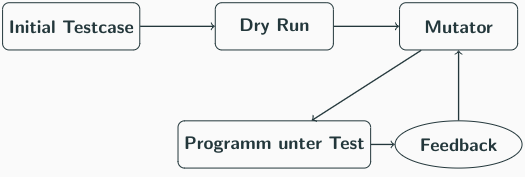
\includegraphics[width=\columnwidth]{res/Struktur_eines_fuzzing_prozesses}
    \caption[Struktur eines Fuzzing Prozesses]{
        Diese Abbildung zeigt den Ablauf eines Fuzzing Prozesses am Beispiel des Fuzzers AFL.
        Der Fuzzer verwendet die bereits gesammelten Testcases.
        Sie werden an das SUT in einer \enquote{Dry Run}-Phase übergeben, um zu überprüfen, ob es durch diese Eingaben
        bereits zum Absturz gebracht werden kann.
        Das Programm wird mit den Eingaben ausgeführt und die Ausgabe wird analysiert.
        Anhand der Analyseergebnisse wird ein Mutator verwendet, um neue Testcases zu generieren, die anhand der initial
        übergebenen Eingaben besonders tief in das Programm eingedrungen sind.
        Die vom Mutator generierten Eingaben werden an das SUT übergeben und das erlangte Feedback des SUT wird zur weiteren
        Verfeinerung der Eingaben verwendet.
        Somit bildet sich ein iterativer Prozess, der die Testcases immer weiter verfeinert.
    }\label{fig:struktur_fuzzing}
\end{figure}
